\chapter{Hierarchical Temporal Memory(HTM)}
\section{HTMの概要}
HTMは大脳皮質の構造と学習アルゴリズムを模して作られたニューラルネットワークである。
構造はカラムとセルによる2次元マップ表現となっており、各セルが状態を偏移させる。
学習アルゴリズムはヘブ則となっており各時刻間で活性化状態のセル同士の接続を強める。
また活性化状態のセルと強く接続しているセルが予測状態に遷移することで予測を行う。

HTMは全部にセルを用いて1つのパターンを表現する。各セルの状態が遷移することで表現するパターンが変化する。

HTMの特徴は時系列データ中の各パターンを再現しつつ学習するためオンライン学習を行っているという点とモデルの訓練とデータの再現を同時に行っているという点がある。
これによって時系列データを連続してモデルに流し続け学習を行うという連続オンライン学習が可能となっている。
また疎な分散表現を用いたことによる並列同時予測が可能な点も挙げられる。

\section{HTMの構造}
HTMの全体構造を下の図2.1に示す。
HTMは複数のカラムの集合となっており、各カラムは複数のセルの集合からなっている。
HTM全体で1つのパターンを表現する。時間が進むごとにパターンが変化していくことで時系列データを表現する。

\begin{figure}[ht]
  \begin{center}
    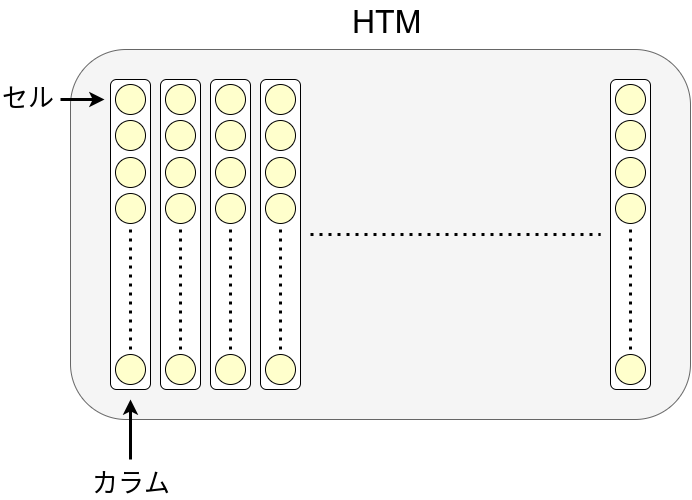
\includegraphics[scale=0.5]{./fig/drawing_1}
    \caption{HTMの全体構造}
    \label{fig:HTM}
  \end{center}
\end{figure}

\subsection{セルの状態変化}
セルの状態は活性化状態と非活性化状態と予測状態の3つであり、各時刻において常にどれか1つの状態を取る。各時刻ごとにそれぞれの状態を相互に遷移する。

\vspace{5mm}
\begin{figure}[ht]
  \begin{center}
    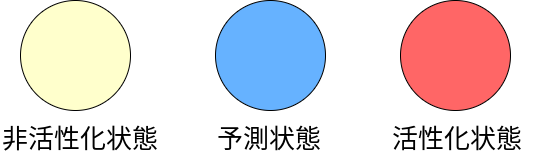
\includegraphics[scale=0.5]{./fig/drawing_2}
    \caption{セルの状態}
    \label{fig:cell_state}
  \end{center}
\end{figure}

\subsection{パターン表現}
HTMはカラムの組み合わせでパターンを表現する。
各カラムにおいてカラム中のセルのどれか1つでも活性化状態になっている場合にそのカラムがパターン表現を構成するカラムとみなす。

\vspace{5mm}
\begin{figure}[ht]
  \begin{center}
    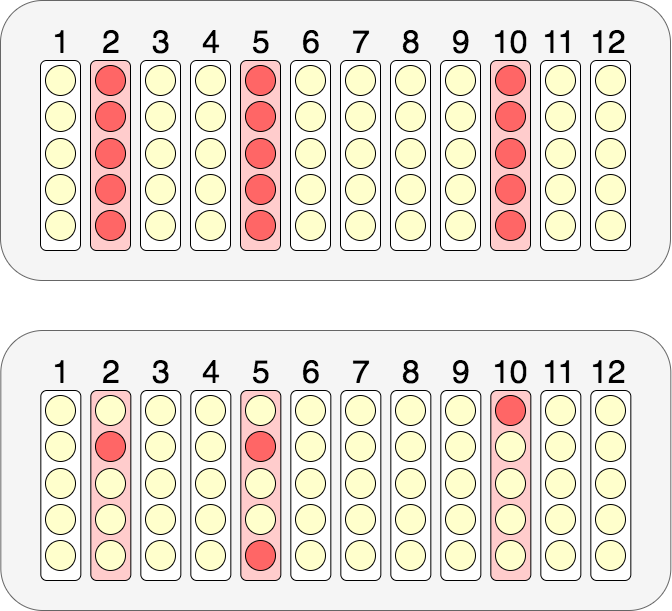
\includegraphics[width=10cm]{./fig/drawing_3}
    \caption{パターンの表現: 上下どちらの図も同じカラムの組み合わせ(2, 5, 10)でパターンを表現しているため、両方同じパターンを表す。}
    \label{fig:pattern_representation}
  \end{center}
\end{figure}

\subsection{セル内の構造}
HTMはセル内にセグメント構造を持っている。
これは大きく分けて2つからなり、入力セグメントとセグメント集合からなる。
入力セグメントは入力を受け取るもので、各セルに1つある。
セグメント集合も各セルに1つあり、接続セグメントを複数持っている。
この接続セグメントは他のセルとの接続値を保持しており、学習によってこの接続値を増減させしきい値との比較によってセル間のシナプス接続を判定する。

\vspace{5mm}
\begin{figure}[ht]
  \begin{center}
    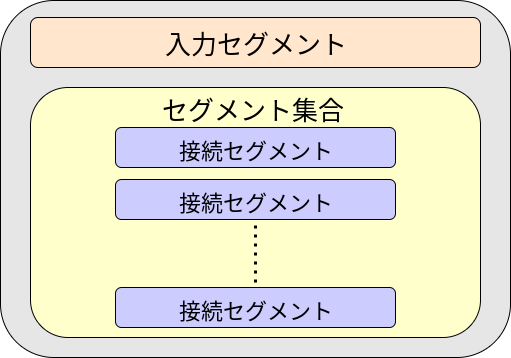
\includegraphics[width=10cm]{./fig/drawing_4}
    \caption{セル内の構造}
    \label{fig:cell_structure}
  \end{center}
\end{figure}

\subsection{疎な分散表現}
学習が進んでいくとHTM中の僅かなセルのみが活性化状態に遷移していき、少ないセルでパターンを表現するようになる。これによって

\section{HTMの学習アルゴリズム}
\subsection{活性化状態の計算}
\subsection{予測状態の計算}
\subsection{セグメント集合を用いた接続値の更新}


\section{HTMの問題点}
\begin{itemize}
  \item 疎な分散表現を用いたために発火するセルが徐々に少なくなり消失する。
  \item 学習が大きく進んだパターンにおいて表現が疎になった時に次のパターンに繋がっていたセルが消失するために学習が損失
\end{itemize}
